\renewcommand*{\arraystretch}{1.1}

\subsection*{Interactive / complex / 4}
\label{section:interactive-complex-read-04}

\renewcommand{\currentQueryCard}{4}
\marginpar{
	\raggedleft
	\vspace{0.22ex}

    \queryRefCard{interactive-complex-read-01}{Interactive}{1}\\
    \queryRefCard{interactive-complex-read-02}{Interactive}{2}\\
    \queryRefCard{interactive-complex-read-03}{Interactive}{3}\\
    \queryRefCard{interactive-complex-read-04}{Interactive}{4}\\
    \queryRefCard{interactive-complex-read-05}{Interactive}{5}\\
    \queryRefCard{interactive-complex-read-06}{Interactive}{6}\\
    \queryRefCard{interactive-complex-read-07}{Interactive}{7}\\
    \queryRefCard{interactive-complex-read-08}{Interactive}{8}\\
    \queryRefCard{interactive-complex-read-09}{Interactive}{9}\\
    \queryRefCard{interactive-complex-read-10}{Interactive}{10}\\
    \queryRefCard{interactive-complex-read-11}{Interactive}{11}\\
    \queryRefCard{interactive-complex-read-12}{Interactive}{12}\\
    \queryRefCard{interactive-complex-read-13}{Interactive}{13}\\
    \queryRefCard{interactive-complex-read-14}{Interactive}{14}\\
}


\noindent\begin{tabularx}{\queryCardWidth}{|>{\queryPropertyCell}p{\queryPropertyCellWidth}|X|}
	\hline
	query & Interactive / complex / 4 \\ \hline
%
	title & New topics
 \\ \hline
%
	pattern & \hfill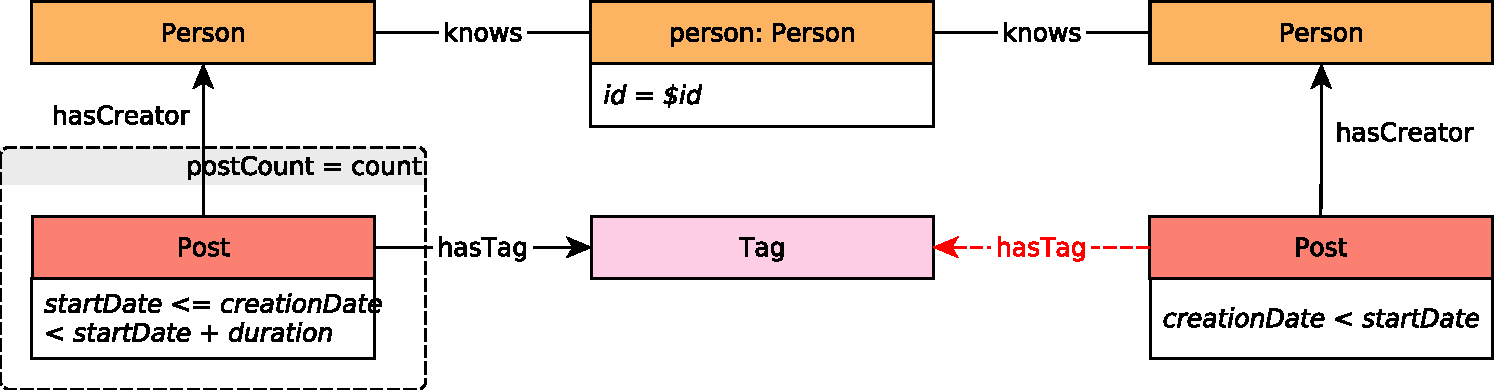
\includegraphics[scale=\patternscale,margin=0cm .2cm]{patterns/interactive-complex-read-04}\hfill\vadjust{} \\ \hline
%
	desc. & Given a start Person, find Tags that are attached to Posts that were
created by that Person's friends. Only include Tags that were attached
to friends' Posts created within a given time interval, and that were
never attached to friends' Posts created before this interval.
 \\ \hline
%
	
		params &
		\innerCardVSpace{\begin{tabularx}{\attributeCardWidth}{|>{\paramNumberCell}c|>{\varNameCell}M|>{\typeCell}m{\typeWidth}|Y|} \hline
		$\mathsf{1}$ & Person.id
 & ID
 &  \\ \hline
		$\mathsf{2}$ & startDate
 & Date
 &  \\ \hline
		$\mathsf{3}$ & duration
 & 32-bit Integer
 & Duration of requested period, in days the interval {[}startDate,
startDate + Duration) is closed-open
 \\ \hline
		\end{tabularx}}\innerCardVSpace \\ \hline
	
%
	
		result &
		\innerCardVSpace{\begin{tabularx}{\attributeCardWidth}{|>{\resultNumberCell}c|>{\varNameCell}M|>{\typeCell}m{\typeWidth}|>{\resultOriginCell}c|Y|} \hline
		$\mathsf{1}$ & Tag.name & String & R &
				 \\ \hline
		$\mathsf{2}$ & count & 32-bit Integer & A &
				Number of Posts made within the given time interval that have this Tag
 \\ \hline
		\end{tabularx}}\innerCardVSpace \\ \hline
	
%
	
		sort		&
		\innerCardVSpace{\begin{tabularx}{\attributeCardWidth}{|>{\sortNumberCell}c|>{\varNameCell}M|>{\directionCell}c|Y|} \hline
		$\mathsf{1}$ & count
 & $\desc
$ &  \\ \hline
		$\mathsf{2}$ & Tag.name
 & $\asc
$ &  \\ \hline
		\end{tabularx}}\innerCardVSpace \\ \hline
	%
	limit & 10 \\ \hline
	%
	CPs &
	\multicolumn{1}{>{\raggedright}l|}{
		\chokePoint{2.3}
		} \\ \hline
	%
	relevance &
		\small This query looks for paths of length two, starting from a given Person, moving to Posts and then to Tags. It tests
the ability of the query optimizer to properly select the usage of hash joins or index based joins, depending on the
cardinality of the intermediate results. These cardinalities are clearly affected by the input Person, the number of
friends, the variety of Tags, the time interval and the number of Posts.
 \\ \hline%
\end{tabularx}
\queryCardVSpace